\documentclass[spanish]{textolivre}

% metadata
\journalname{Texto Livre}
\thevolume{17}
%\thenumber{1} % old template
\theyear{2024}
\receiveddate{\DTMdisplaydate{2024}{2}{19}{-1}}
\accepteddate{\DTMdisplaydate{2024}{2}{27}{-1}}
\publisheddate{\today}
\corrauthor{Alberto Luis García García}
\articledoi{10.1590/1983-3652.2024.51273}
%\articleid{NNNN} % if the article ID is not the last 5 numbers of its DOI, provide it using \articleid{} commmand 
% list of available sesscions in the journal: articles, dossier, reports, essays, reviews, interviews, editorial
\articlesessionname{articles}
\runningauthor{García García et al.}
%\editorname{Leonardo Araújo} % old template
\sectioneditorname{Hugo Heredia Ponce}
\layouteditorname{João Mesquita}

\title{El autoaprendizaje aplicado a las asignaturas de tecnología audiovisual. Estudio de caso}
\othertitle{Autoaprendizagem aplicada a disciplinas de tecnologia audiovisual. Estudo de caso}
\othertitle{Self-learning applied to audiovisual technology subjects. Case study}

\author[1]{Alberto Luis García García~\orcid{0000-0002-6805-6700}\thanks{Email: \href{mailto:algarci@ucm.es}{algarci@ucm.es}}}
\author[2]{Manuel Sánchez Cid~\orcid{0000-0002-7683-9000}\thanks{Email: \href{mailto:manuel.cid@urjc.es}{manuel.cid@urjc.es}}}
\author[3]{Fernando Marroquín-Ciendúa~\orcid{0000-0002-2213-4566}\thanks{Email: \href{mailto:fernando.marroquinc@utadeo.edu.co}{fernando.marroquinc@utadeo.edu.co}}}
\affil[1]{Universidad Complutense de Madrid, Madrid, España.}
\affil[2]{Universidad Rey Juan Carlos, Madrid, España.}
\affil[3]{Universidad de Bogotá Jorge Tadeo Lozano, Bogotá, Colombia.}


\addbibresource{article.bib}
\usepackage{multirow}
\usepackage{tabularx}
\usepackage{array}


\begin{document}

\renewcommand{\tabularxcolumn}[1]{m{#1}}
%Faz com que toda coluna X passe de tipo p, para tipo m. Supostamente isso faz com que sejam alinhadas verticalmente, mas não percebo. Talvez um erro?
\maketitle
\begin{polyabstract}
\begin{abstract}
El presente trabajo pretende demostrar, a través de un estudio de caso, las necesidades de aprendizaje en una asignatura práctica perteneciente al grado de Comunicación Audiovisual de la Universidad Complutense de Madrid, para comprobar las posibilidades que ofrece el autoaprendizaje como complemento a la formación presencial. El principal objetivo del estudio es analizar la percepción del alumnado sobre la adquisición de conocimientos a través de estrategias de autoaprendizaje dentro de la asignatura tecnológica experimental denominada "Edición y Postproducción". Para ello se ha realizado una investigación cuantitativa, exploratoria, descriptiva y relacional con una muestra de 154 participantes, según un cuestionario con tres categorías de análisis centrado en: 1) formación y aprendizaje, 2) dedicación y métodos de trabajo, y 3) resolución y ayuda complementaria. Los resultados obtenidos permiten extraer conclusiones sobre la idoneidad del proceso formativo actual, las necesidades que implican el aprendizaje y la utilidad de un sistema formativo de autogestión para complementar la formación presencial. 

\keywords{Enseñanza centrada en el desempeño \sep Aprendizaje personalizado \sep Tecnologías de la información \sep Auto aprendizaje \sep Aprendizaje activo}
\end{abstract}

\begin{portuguese}
\begin{abstract}
Este artigo pretende demonstrar, através de um estudo de caso, as necessidades de aprendizagem numa disciplina prática pertencente ao curso de Comunicação Audiovisual da Universidade Complutense de Madrid, a fim de verificar as possibilidades oferecidas pela auto-aprendizagem como complemento da formação em sala de aula. O objetivo principal do estudo é analisar a percepção dos alunos sobre a aquisição de conhecimentos através de estratégias de auto-aprendizagem na disciplina tecnológica experimental denominada "Edição e Pós-produção". Para o efeito, foi realizada uma investigação quantitativa, exploratória, descritiva e relacional com uma amostra de 154 participantes, segundo um questionário com três categorias de análise centradas em: 1) formação e aprendizagem, 2) dedicação e métodos de trabalho e 3) resolução e ajuda complementar. Os resultados obtidos permitem tirar conclusões sobre a adequação do processo de formação atual, as necessidades de aprendizagem e a utilidade de um sistema e formação autogerido para complementar a formação presencial. 

\keywords{Ensino centrado no desempenho \sep Aprendizagem personalizada \sep Tecnologias da informação \sep O ensino centrado no desempenho}
\end{abstract}
\end{portuguese}

\begin{english}
\begin{abstract}
The aim of this paper is to present, through a case study, the learning needs in a practical subject included in the Audiovisual Communication degree at the Complutense University of Madrid. The aim is to verify the possibilities offered by self-learning as a complement to classroom teaching. The main objective of the study is to analyse the students' perception of the acquisition of knowledge through self-learning strategies within the experimental technological subject called "Editing and Postproduction". For this purpose, a quantitative, exploratory, descriptive and relational research has been carried out with a sample of 154 participants, according to a questionnaire with three categories of analysis focused on: 1) training and learning, 2) commitment and working methods, and 3) resolution and additional help. The results will allow conclusions to be drawn about the adequacy of the current training process, the learning needs and the usefulness of a self-management training system as a complement to classroom training.

\keywords{Performance-centred teaching \sep Personalised learning \sep Information technology \sep Self-learning \sep Active learning}
\end{abstract}
\end{english}
\end{polyabstract}

\section{Introducción}
En la mayoría de los actuales planes de estudio de Comunicación Audiovisual de las Facultades de Ciencias de la Comunicación españolas (año 2024), se evidencia una escasa asignación temporal en las asignaturas tecnológicas de corte práctico. Casi como norma, las universidades implementan dichas asignaturas en un cuatrimestre, lo que equivale de media a 28 horas lectivas de teoría y 28 horas lectivas de práctica; además se ven reducidas a un tiempo efectivo de 21 horas en cada parte como consecuencia del tiempo de descanso descontado. 

Esta limitación temporal es recurrente desde la aplicación del modelo incluido en el \textit{Libro Blanco de los Títulos de Grado en Comunicación} \cite{agencia_nacional_de_evaluacion_de_la_calidad_y_acreditacion_titulos_2005} (ANECA), siendo una problemática que no parece encontrar una solución tangible. Por ello, el concepto de autoaprendizaje se convierte en un recurso alternativo valorable, ya sea mediante mecanismos estructurados por el docente, bien por procesos voluntarios del alumnado o como mezcla de ambos. Dentro de este concepto de autoaprendizaje en asignaturas tecnológicas prácticas, resultará interesante considerar las oportunidades que ofrecen los sistemas de realimentación constructiva, como la IA, ya que permite proyectar una evolución adaptativa y personalizada del aprendizaje, aunque para este tipo de materias aún no se ha hecho realidad.

Pero esta propuesta de fomentar el autoaprendizaje en asignaturas tecnológicas no es algo nuevo, ya que, distintos modelos educativos reconocidos a nivel internacional como la integración de la enseñanza en remoto con la presencial, denominado “aprendizaje mixto” (\textit{blended learning}), o el sistema en el que el alumnado prepara activa y previamente el desarrollo de los contenidos de la materia con la supervisión del profesorado, lo que se conoce como “clase invertida” (\textit{flipped classroom}), así como el aprendizaje basado en proyectos, promueven la estimulación y el interés activo del estudiantado mediante una puesta en escena vinculada netamente con la autogestión del aprendizaje. En el caso del \textit{flipped classroom}, para \textcite[307]{mejon_opiniones_2018}, “las personas aprenden mejor cuando están comprometidas, por lo que la clase invertida abre un camino sostenible de aprendizaje que alterna el trabajo previo a las clases, en el aula, y actividades después las clases”. En el aprendizaje basado en proyectos, se demanda igualmente una iniciativa, implicación y gestión personalizada por parte del alumnado, que trasciende la pauta docente generada en el aula.

En el caso de las asignaturas tecnológicas de corte práctico de Ciencias de la Comunicación, éstas, se ven abocadas a asumir directamente la transformación derivada del incesante desarrollo tecnológico promovido por los medios y empresas del sector, lo que conlleva por necesidad, una constante renovación de los programas formativos y de sus herramientas. La realidad profesional nunca debería quedar al margen del ámbito formativo universitario, pero este conocimiento debe entenderse desde una perspectiva constructivista de índole global y no como formación específica aislada centrada únicamente en la instrumentación tecnológica. Estos nuevos perfiles tienen en común la necesidad de un alto grado de conocimiento y especialización tanto en su filosofía analítica y creativa como en la operativa instrumental. Las facultades de Ciencias de la Comunicación no deberían quedar al margen de esta evolución tecnológica, entendiendo que éstas tampoco deben convertirse en un espacio exclusivo para la formación técnica, debiendo potenciar la adquisición de conocimiento relacional, la investigación y, por supuesto, la motivación para la generación de pensamiento analítico y crítico. Atendiendo a lo anterior, en esta investigación se defiende una formación para las asignaturas de corte tecnológico que sea rigurosa, expansiva en su conocimiento, habilitadora de capacidades profesionales y que fomente la reflexión, considerando por ello oportuna la aportación de \textcite{besalu-casademont_competencias_2017} cuando afirma que la universidad debe decidir entre la introducción constante de competencias tecnológicas en su formación o derivar hacia competencias más generales que permitan a los egresados adaptarse al constante cambio tecnológico. 

Es innegable que, en el ámbito universitario, el análisis profundo y la reflexión deben ser parte esencial en la gestión del conocimiento, pero resulta fundamental focalizar la observación en su contexto y no como una generalidad aplicable a todas las materias y asignaturas. Es decir, la discusión debería plantearse sobre la planificación de un modelo formativo que contemple verdaderamente las necesidades instrumentales y de asignación temporal en este tipo de formación. Volviendo al concepto del autoaprendizaje como apoyo y solución factible ante la actual limitación temporal asignada por los planes de estudio universitarios de Ciencias de la Comunicación para este tipo de asignaturas, entre los distintos recursos complementarios está el uso de tutoriales ubicados en la red junto a las aplicaciones capaces de optimizar los procesos de producción, lo que está convirtiendo a este tipo de herramientas en auténticos asistentes técnico-formativos. 

En este sentido, aunque tanto el cuerpo docente como el alumnado se convierten en numerosas ocasiones en solventes generadores de contenidos audiovisuales de carácter formativo, tal y como indica \textcite{alcala_del_olmo_fernandez_competencias_2020} en \textcite[p. 2]{garcia-penalvo_evaluacion_2020}, también se dan casos de “una brecha de competencias, relacionada con las competencias digitales del profesorado y del estudiantado para utilizar adecuadamente las plataformas digitales con fines educativos y la capacidad de crear o proveer contenidos y actividades educativas a través de estas”. Pero esta producción de contenidos formativos no es exclusiva de las partes anteriormente citadas, ya que las propias compañías tecnológicas, así como distintos profesionales del sector, han acreditado la validez y utilidad de sus aportaciones, tanto para su uso en el aula como en la gestión particular del aprendizaje.

Por otra parte, aunque para los autores resulta incuestionable que las asignaturas dedicadas a las tecnologías audiovisuales requieren de un compromiso de autoaprendizaje y autogestión extra para la adquisición del conocimiento de las teorías, experiencias, aplicaciones, programas y herramientas que configuran el currículum de estas asignaturas, este requerimiento de autoaprendizaje se encuentra con un problema añadido, tal y como afirma \textcite{mejon_opiniones_2018}, %Mejón et al. (2018),
dándose una disparidad en el nivel de conocimientos sobre tecnología entre el alumnado.

A su vez, la problemática va más allá de la citada circunstancia. Aunque pueda resultar chocante, a pesar de establecerse un programa de asignatura más o menos estandarizado a nivel nacional, la formación aplicada por el profesorado también puede variar dependiendo del centro, del profesorado e incluso del turno en el que se imparte la asignatura. Estas variables son susceptibles de generar desajustes en la concepción, organización y desarrollo de los programas formativos, lo que a su vez puede incrementar las divergencias a la hora de solventar las limitaciones existentes. 

En opinión de los autores, la consolidación de mecanismos de autoaprendizaje parece ser la solución más plausible para el óptimo desarrollo del proceso formativo en estas materias de carácter tecnológico. Por ello, y en busca de elementos objetivos que permitan acreditar la fortaleza y necesidad del autoaprendizaje como resorte formativo, el presente trabajo se asienta en el resultado de una primera fase de la investigación que venimos desarrollando en el Grado de Comunicación Audiovisual de la Universidad Complutense de Madrid para evidenciar la percepción sobre el actual modelo formativo. 

El autoaprendizaje está activo en dos direcciones: la del profesorado hacia otros colegas y el alumnado, y la del alumnado hacia las nuevas posibilidades de adquisición de conocimiento y competencias. \textcite{alcala_del_olmo_fernandez_competencias_2020} han comprobado que el uso de aplicaciones y recursos digitales amplifica las oportunidades de crecimiento profesional gracias a la capacidad para conectar con otros colegas con intereses similares en lo que denominan “Personal Learning Networks" (PLN) y, de esta manera, generar contenidos colaborativos que potencian la diversidad y la complementariedad en el aprendizaje de contenidos específicos por parte del alumnado. En la dirección contraria, el alumnado en su proceso de aprendizaje activo entra en una dinámica de constante intercambio de opiniones e ideas, propuesta de preguntas concretas sobre conceptos específicos, etc., que llevan a un proceso de aprendizaje más parecido a un sistema conversacional que a la aptitud de escucha presente en el aula. En esta línea, postulada por \textcite{prestridge_categorising_2019}, se desarrolla la colaboración activa entre estudiantes a través de los medios en los que se comparten conocimientos, como las herramientas sociales de comunicación, estimulando una cultura de colaboración en la que a través de aspectos informales aprenden la importancia del trabajo en equipo, de la comunidad y el valor de la corresponsabilidad funcional. 

El desarrollo anterior permite establecer como hipótesis de partida que, atendiendo al actual escenario de formación basado en la docencia presencial a un número de alumnos elevado, medios técnicos escasos y una asignación temporal limitada frente a la totalidad de la materia a impartir, la autoformación personalizada apoyada en contenidos extra ubicados en fuentes externas a la sesión presencial, posibilita evolucionar hacia procesos de aprendizaje complementarios que facilitan un mayor desarrollo formativo, tanto en las rutinas diarias de la materia, como en la percepción de actividades académico-profesionales. Así mismo, junto al objetivo principal, centrado en recabar entre el alumnado su valoración respecto al concepto de autoaprendizaje y sobre las herramientas empleadas en su desarrollo, se establece como objetivo secundario, pero no menos importante, detectar mediante el análisis de un caso aplicado, aquellos aciertos y carencias que permitan definir aspectos metodológicos que optimicen el proceso de aprendizaje.

En definitiva, esta investigación pretende medir la valoración del estudiantado sobre distintos aspectos reseñables entroncados con el proceso de aprendizaje en esta formación técnica específica, considerando fundamental ahondar en aquellos elementos que permitan verificar este nuevo escenario relacionado con técnicas de innovación educativa conforme al autoaprendizaje automático. 

Al objeto de verificar nuevas rutinas formativas centradas en el uso de tecnologías educativas que tienen en el autoaprendizaje su principal esencia, se aportan los resultados obtenidos mediante un cuestionario realizado a una muestra representativa dentro de la Facultad de Ciencias de la Información de la Universidad Complutense de Madrid, compuesta por estudiantes matriculados en la asignatura tecnológica de corte práctico con mayor número de matriculados en la titulación de Comunicación Audiovisual, siendo la asignatura: Edición y Postproducción.

\section{Materiales y métodos}\label{sec-normas}
El presente estudio contó con una fase exploratoria de corte cualitativo y otra fase cuantitativa a través de encuestas en la que se buscó observar relaciones entre variables, mediante la aplicación de la prueba Chi 2. La fase cualitativa fue realizada con un muestreo por conveniencia con treinta (30) estudiantes participantes a través de entrevistas en profundidad y tres grupos focales con seis (6) participantes cada uno. Para ello se configuró un instrumento semiestructurado indagando en aspectos relacionados con las siguientes variables: psicográficas, aprendizaje a través de las TIC, didáctica, autoaprendizaje y trabajo en equipo.  A partir de aquí se permitió establecer tres categorías o ejes de indagación, que conformaron el instrumento de la fase cuantitativa final. Estos fueron: 1- formación técnica y conocimiento / aprendizaje; 2- dedicación y modo de trabajo; 3- resolución de ejercicios y ayuda complementarias. De acuerdo con lo anterior, se dispuso un instrumento validado cognitivamente por un grupo de estudiantes y mediante juicio de expertos, siendo este último formado por un grupo de cinco profesionales con una doble experiencia mayor a diez años tanto en los medios audiovisuales como en la actividad docente universitaria. 

El material se compuso de un apartado que indagaba sobre el perfil del estudiante, y tres categorías de indagación -mencionados anteriormente y emergentes de la fase exploratoria cualitativa- formando un total de 22 variables. Todas ellas relacionadas de una u otra forma con el proceso de enseñanza-aprendizaje aplicado en la asignatura seleccionada. Estas variables fueron medidas a través de escalas dicotómicas (síno), de selección múltiple y preguntas abiertas. La asignatura en la cual se centró el estudio fue Edición y Postproducción de cuarto curso del Grado de Comunicación Audiovisual de la Facultad de Ciencias de la Información de la Universidad Complutense de Madrid. 

Los ejes de indagación y variables especificadas en el instrumento aplicado a través de la encuesta estructurada, se presentan en la \Cref{tab-01}.

%Tabla 1
\begin{table}[h]
\centering\small
\begin{threeparttable}
\caption{Categorías de estudio.}
\label{tab-01}
\begin{tabular}{p{3cm} l p{10cm}}
\toprule
Categorías & \# & Variables \\
\midrule
\multirow[t]{6}{=}{1.Demográficas/ Localización} & 1 & Edad\\
	 & 2 & Género \\
	 & 3 & Grado que se cursa actualmente \\
	 & 4 & Curso matriculado\\
	 & 5 & Asignatura matriculada\\
  & 6 & Turno\\[2ex]
\multirow[t]{7}{=}{2. Formación técnica y conocimiento-aprendizaje} & 7 & Necesidad de utilización de herramientas técnicas para el aprendizaje\\
  & 8	& Opinión sobre la necesidad de formación técnica sobre software\\
  & 9	& Opinión sobre la formación técnica impartida según objetivos\\
  & 10 &Valoración del aprendizaje de herramientas tecnológicas\\
  & 11  & Nivel de conocimiento alcanzado con el software\\
  & 12 & Facilidad de entendimiento en relación con herramientas del software\\
  & 13 & Dificultad de entendimiento en relación con aplicaciones del software\\[4ex]
\multirow[t]{4}{=}{3. Dedicación y modo de trabajo} &  14 & Forma de trabajo en clase (individual, parejas)\\
  & 15 & Estimación de dedicación de horas prácticas para aprendizaje de software en clase\\
  & 16 & Dedicación de horas prácticas fuera de clase\\
  & 17 & Dedicación para resolución de ejercicios\\[2ex]
\multirow[t]{5}{=}{4. Resolución de ejercicios y ayuda complementaria} & 18 & Opinión sobre necesidad de licencias individuales fuera de aula \\
  & 19 & Dedicación temporal a resolver el ejercicio o a pensar en las operaciones para su resolución\\
  & 20 & Preferencias sobre tipos de ayuda para resolver problemas técnicos y ejercicios prácticos\\
  & 21 & Empleo de tutoriales como complemento a la clase\\
  & 22 & Opinión sobre la necesidad de utilizar ayuda online\\	
\bottomrule
\end{tabular}
\source{Elaboración propia.}
\end{threeparttable}
\end{table}

\subsection{Participantes}\label{sec-conduta}
\textit{Fase exploratoria cualitativa} 

Se utilizó un muestreo por conveniencia en el que se seleccionaron estudiantes de diferentes cursos, con un total de treinta (30) estudiantes para las entrevistas y seis (6) estudiantes para cada grupo focal. En total hubo tres grupos focales. Las edades de los participantes estaban en el rango de 18 a 23 años y su género estaba repartido proporcionalmente.  

\textit{Fase cuantitativa encuestas}

Para la selección de la muestra se realizó un muestreo no probabilístico por conveniencia, estando compuesta por estudiantes de la asignatura seleccionada para el estudio. Se tuvo en cuenta el total de la población de estudiantes del grado de Comunicación Audiovisual que cursaban la asignatura “Edición y Postproducción” de la Universidad Complutense de Madrid. Así, para una muestra representativa con un nivel de confianza = 99~\% y margen de error = 5~\% fueron seleccionados 154 estudiantes \cite{sucasaire_pilco_orientaciones_2022,hernandez_sampieri_metodologiinvestigacion_2018}. Se ha estimado un universo de 193 estudiantes, siendo estos los correspondientes al total de matriculados en la asignatura de Edición y Postproducción de 4º curso de Comunicación Audiovisual de la Facultad de Ciencias de la Información de la citada Universidad. El número de encuestas realizadas pertenecientes al grado y a la asignatura objetos del estudio es de 154, lo que supone un 80~\% del total del estudiantado matriculado en la misma y un 22,5~\% del total del alumnado matriculado en el grado de Comunicación Audiovisual.


\subsection{Justificación de la asignatura}\label{sec-fmt-manuscrito}
La elección de la asignatura de Edición y Postproducción de cuarto curso del grado en Comunicación Audiovisual, se fundamenta en los siguientes aspectos: en primer lugar, por ser una asignatura de último curso, lo que facilita una muestra con una mayor perspectiva y experiencia en el proceso de aprendizaje desarrollado a lo largo de los estudios; en segundo lugar, por ser la asignatura de corte tecnológico experimental en dicha facultad que incorpora en su Guía Docente la utilización de un mayor número de programas o herramientas digitales de trabajo centradas en el tratamiento de la señal audiovisual en las salas multimedia; y, en tercer lugar, por ser el número de matriculados en la asignatura elegida para el estudio, el mayor de la citada titulación, representando los resultados del ejercicio aquí descrito un 80~\% sobre el total de alumnos matriculados en la asignatura y un 22,5~\% del total de matriculados en la titulación\footnote{\url{https://ccinformacion.ucm.es/estudios/2023-24/grado-comunicacionaudiovisual-plan-803773}}. Aunque en esta primera fase se ha focalizado el trabajado sobre los estudiantes que cursaban esta asignatura, la intención es extrapolar el estudio a las asignaturas similares en los programas de los Grados de otros centros universitarios.


\subsection{Procedimiento}\label{sec-formato}
El procedimiento está dividido en los siguientes apartados: instrumentos, perfil de los estudiantes encuestado, categorías y aportación al conocimiento. 


\subsubsection{Instrumentos}\label{sec-modelo}
El cuestionario se construyó mediante la herramienta Google Forms, previa evaluación de expertos –docentes y profesionales del sector audiovisual- y teniendo en cuenta la pertinente información exploratoria y documental para la construcción de categorías y variables. Posteriormente se validó a través de una prueba piloto con treinta estudiantes para conocer el nivel de entendimiento, pertinencia y comprensión de las preguntas y de las escalas de medición planteadas. Conforme a los objetivos del estudio, el formulario desarrolla una encuesta estructurada, siendo cumplimentada por el alumnado durante las sesiones presenciales de clase, bajo la supervisión de un docente y durante un periodo de tres meses. Para el procesamiento, análisis de los datos y resultados descriptivos y de relación entre las variables, se utilizó la prueba Chi 2 mediante el uso del software SPSS versión 25.

\subsubsection{Perfil de estudiantes encuestados}\label{sec-organizacao}
En esta sección las preguntas se establecen para confirmar la pertenencia de los encuestados a la titulación, curso y asignatura, siendo en el presente caso: Comunicación Audiovisual, 4º curso y la asignatura de Edición y Postproducción. En el caso de las preguntas sobre el Grado y la asignatura matriculada en el momento de la encuesta, sirven para ratificar la validez de los datos obtenidos y excluir del estudio aquellos cuestionarios que incumplan con las respuestas establecidas como requisitos, siendo necesario estar cursando la asignatura de Edición y Postproducción y el Grado en Comunicación Audiovisual. La muestra se conformó por rangos de edad y género, con un criterio de inclusión referente a que fueran estudiantes de Comunicación Audiovisual y que estuvieran cursando la asignatura de Edición y Postproducción, tal y como se indica en la \Cref{tab-02}.

%Tabla 2
\begin{table}[h]
\centering\small
\begin{threeparttable}
\caption{Perfil de los participantes.}\label{tab-02}
\begin{tabular}{lp{10cm}}
\toprule
Variabel & Atributos\\
\midrule
\multirow[t]{3}{*}{Edad (rangos de edad)} & 21 años: 68,8~\% \\
  & 22 años: 13,6~\% \\
  & Más de 23 años: 17,6~\% \\[2ex]
\multirow[t]{3}{*}{Género} & Mujer: 60,4~\% \\
  & Hombre: 39,6~\% \\
  & Otros: 0,6~\% \\[2ex]
\multirow[t]{3}{*}{Turnos de estudio} & Turno de mañana: 53,6~\% \\
  & Turno de tarde: 24,8~\% \\
  & Turno compartido (matriculados en asignaturas de ambos turnos): 21,6\\
\bottomrule
\end{tabular}
\source{Elaboración propia.}
\end{threeparttable}
\end{table}

\subsubsection{Categorías}\label{sec-organizacao-latex}

\begin{enumerate}
    \item Necesidad de formación, aprendizaje y conocimiento técnico relativo a las herramientas vistas en la asignatura. Esta categoría, indaga sobre la importancia otorgada al uso y relación de las tecnologías con respecto al aprendizaje de la asignatura objeto de estudio, así como permite establecer interrelaciones de verificación y contraste entre las variables de otras categorías. 
    \item Dedicación en tiempo y modo de trabajo. En esta categoría, se analiza el proceso temporal necesario para el aprendizaje de las herramientas técnicas vistas en la asignatura, centrándose en la estimación temporal para el aprendizaje. 
    \item Resolución de ejercicios y ayuda complementaria. Aquí se observan las preferencias sobre tipos de ayuda y empleo de herramientas para el autoaprendizaje.
\end{enumerate}

\subsubsection{Aportación al conocimiento}\label{sec-titulo}
Esta investigación se desarrolla con la pretensión de aportar datos contrastados suficientes que evidencien el estado de la cuestión a nivel formativo de las asignaturas tecnológicas de corte práctico-experimental de Edición y Postproducción, y el subsiguiente proceso de enseñanza-aprendizaje. A su vez, el trabajo inquiere en la valoración que concede el alumnado al autoaprendizaje mediante el uso de tecnologías educativas personalizadas en red como complemento formativo. Ambas cuestiones se consideran relevantes por la trascendencia de las conclusiones, pudiendo significar una visión constructiva frente a posibles limitaciones estructurales. 

\section{Análisis y resultados}\label{sec-autores}
\subsection{Relaciones con el género}
En los análisis inferenciales de la investigación, se establecieron relaciones entre las variables género y las variables sobre manejo y aprendizaje de \textit{software}, además de otras asociaciones entre categorías de análisis de interés para los objetivos del estudio: manejo de \textit{software} vs. aprendizaje en el aula y autónomo; \textit{software} de la asignatura vs. aprendizaje autónomo y, aprendizaje en el aula vs. aprendizaje autónomo. En lo referente a las variables asociadas a la utilización del \textit{software} se observó que el género presenta una relación significativa con el “nivel de conocimientos alcanzados”.

Según los hallazgos incluidos en la \Cref{tab-03}, se observa que el 49,5~\% de los hombres perciben como “suficiente” el nivel de conocimiento alcanzado con el \textit{software} que se enseña en la asignatura, mientras, las mujeres reflejan un 51,7~\%. No obstante, se evidencia que un 30,1~\% de los hombres lo conciben como “bueno”, frente al 23,3~\% de las mujeres ($\chi^{2}(3,N=153)=10.295$, $p=0.016$). Aunque se esperaría un mayor nivel de conocimiento en ambos géneros, estos resultados estarían reflejando que esta variable podría incidir en cómo se asume el aprendizaje técnico por parte de hombres y mujeres. Al mismo tiempo, se observó que al 40,0~\% de las mujeres les resulta fácil entender la interfaz, en contraste con apenas el 16,1~\% de los hombres ($\chi^{2}(1,N=153)=10.942$, $p=0.001$). Por otro lado, respecto a la dificultad de entender el \textit{software} para trabajar, se observó que a los hombres (57,0~\%) les resulta más complicado que a las mujeres (38,3~\%) entender lo relacionado al trabajo con sonido ($\chi^{2}(1,N=153)=5.078$, $p=0.024$). 

%Tabla 3
\begin{table}[htpb]
\centering\small
\begin{threeparttable}
\caption{Asociaciones significativas con el Género.}
\label{tab-03}
\begin{tabular}{p{5cm}*{4}{l}}
\toprule
Variable & Opinión	& Hombre & Mujer & Prueba de asociación\\
\midrule
\multirow[t]{2}{=}{Nivel de conocimiento alcanzado con el software (Avid, Mistika) que se enseña en la asignatura} & Suficiente & 49,5~\%	& 51,7~\% & \begin{tabular}[t]{@{}l@{}}$\chi^{2}(3,N=154)=10,295$\\$\rho=.016$\end{tabular} \\
  & Bueno & 30,1\% & 23,3\% & \\[2ex]
Facilidad de entender la interface & Fácil & 16,1\% & 40,0\% & \begin{tabular}[t]{@{}l@{}}$\chi^{2}(1,N=154)=10,942$\\$\rho<.001$\end{tabular} \\[2ex]
Dificultad de entender el software (Avid, Mistika) referente  al trabajo con sonido & Con dificultad & 57,0~\% &	38,3~\% & \begin{tabular}[t]{@{}l@{}}$\chi^{2}(1,N=154)=5,078$ \\$\rho=.024$\end{tabular} \\
\bottomrule
\end{tabular}
\source{Elaboración propia.}
\end{threeparttable}
\end{table}

En lo referente al turno de estudio (\Cref{tab-04}), los datos resultantes muestran que la jornada en la que los estudiantes realizan sus actividades académicas está relacionada significativamente con el nivel de conocimientos alcanzados. Aquí los del turno de la mañana muestran buenos niveles de conocimientos alcanzados (56.1~\%) ($\chi^{2}(6,N=153)=14.317)$, $p=0.026)$.  Del mismo modo, este mismo alumnado del turno de la mañana (60,8~\%), considera que se imparte suficiente formación técnica de acuerdo con los objetivos de la asignatura. Esto, contrasta con la mayoría del alumnado del turno de tarde (34,2~\%), quien tiene una apreciación negativa respecto a la suficiencia de formación técnica impartida ($\chi^{2}(2,N=153)=7.843$, $p=0.020$). 

%Tabla 4
\begin{table}[htpb]
\centering\small
\begin{threeparttable}
\caption{Asociaciones significativas con el turno de estudio.}
\label{tab-04}
\begin{tabular}{p{5cm}*{4}{l}}
\toprule
Variable & Opinión & Mañana & Tarde & Prueba de asociación\\
\midrule
\multirow[t]{2}{=}{Nivel de conocimientos alcanzado con el software  (Avid, Mistika) enseñado} & Bueno & 56,1~\% & 17,1~\% &
	\begin{tabular}[t]{@{}l@{}}$\chi^{2}(6,N=154)=14,317$ \\ $\rho=.026$\end{tabular} \\
  & Suficiente & 48,7~\% & 35,9~\% & \\[2ex]			
Percepción sobre la formación técnica de acuerdo con los objetivos de las asignaturas & Suficiente & 60,8~\% & 14,9~\% & 
    \begin{tabular}[t]{@{}l@{}}$\chi^{2}(2,N=154)=7,843$ \\ $\rho=.020$\end{tabular} \\
\bottomrule
\end{tabular}
\source{Elaboración propia.}
\end{threeparttable}
\end{table}


\subsection{Necesidad de formación, aprendizaje y conocimiento técnico relativo a las herramientas vistas en la asignatura}\label{sec-idioma}
Esta segunda categoría se centra en la consideración o importancia que concede la muestra al uso de herramientas técnicas, así como al nivel de formación, conocimiento y aprendizaje adquirido con relación a dichas herramientas de la asignatura. En lo que respecta a la “necesidad de utilizar herramientas técnicas para el aprendizaje de la asignatura” (pregunta 7), se evidencia que el 100~\% de la muestra considera necesario utilizarlas. De manera similar, el 94,2~\% considera necesaria la formación técnica de las distintas herramientas de la asignatura, mostrando una concordancia mayoritaria según la necesidad de empleo de herramientas técnicas.  

Si atendemos a la opinión sobre la formación técnica según los objetivos establecidos en la asignatura, los resultados aportan un ligero valor negativo, al considerar como insuficiente la formación técnica de la asignatura en un 51,9~\%. Por su parte, el 48,1~\% la considera suficiente. En cuanto al nivel de aprendizaje adquirido respecto a las herramientas técnicas de la asignatura utilizadas en las salas multimedia, se pudo observar que el 88,4~\% denotó un concepto positivo. Esto, coincide en esencia con los resultados dentro de los conocimientos alcanzados, donde un 81,2~\% considera como positivo el nivel alcanzado con las herramientas técnicas que se enseñan en la asignatura. Sin embargo, contrasta con los resultados observados en lo referente a la opinión sobre la formación técnica, ya que el 51,9~\% la considera insuficiente conforme a la \Cref{fig1}.

\begin{figure}[h!]
\centering
\begin{minipage}{.8\textwidth}
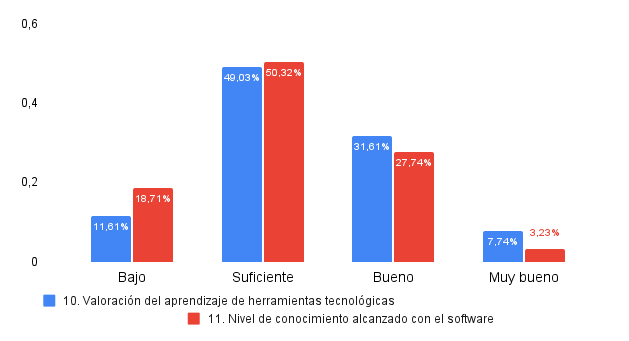
\includegraphics[width=\linewidth]{Fig1.png}
\caption{Valoración del aprendizaje por parte del alumnado.}
\label{fig1}
\source{Elaboración propia.}
\end{minipage}
\end{figure}

En relación con la percepción sobre la facilidad de entendimiento de las herramientas que ofrece el \textit{software} (pregunta 12), los resultados sobre las distintas operaciones que la muestra considera como más fáciles dentro de los programas vistos en la asignatura, se concentran en estas cuatro variables al ser las más representativas conforme a la coincidencia acumulada: a) creación de proyecto, con un 76~\%, b) configuración básica, con un 61~\%, c) operación básica, con un 56,5~\%, y d) guardar proyecto, con un 55,2~\%.

Contrario a lo anterior y en lo referente a las dificultades de entendimiento de las herramientas presentes en el \textit{software}, los hallazgos muestran cuatro resultados más significativos conforme a la coincidencia acumulada: a) ecualizar (sonido), con un 62,3~\%, b) corrección de color (vídeo), con un 48,1~\%, c) formatos (vídeo y sonido), con un 43,5~\%, y d) mezclar sonido (sonido), con un 35,7~\%. Asimismo, respecto a los conceptos genéricos referidos a la dificultad en los procesos de orden general, se indican los siguientes resultados descriptivos: a) trabajar sonido, con un 50~\%, b) postproducir (vídeo y sonido), con un 39~\%, y c) trabajar vídeo, con un 25,3~\%. Así, Los resultados globales describen un nivel de dificultad de entendimiento semejante tanto en la parte de vídeo como en la de sonido. No obstante, se observa que los procesos relacionados con el sonido encabezan el nivel de dificultad.

\subsection{Dedicación en tiempo y modo de trabajo}\label{sec-resumo}
Esta categoría de análisis indaga sobre la dedicación temporal y el modo de trabajo asignado para el aprendizaje de las herramientas tecnológicas vistas en la asignatura. Los resultados respecto a las preferencias sobre la forma de trabajo en clase (individual o parejas) en relación con el aprendizaje, otorgan una clara prioridad al trabajo en pareja, reflejando un 65~\% de preferencia. En la misma línea de análisis, respecto a la percepción que el alumnado tiene sobre la cantidad de tiempo necesario para optimizar su formación, el planteamiento se divide en: a) la estimación de horas prácticas que se necesitan para el aprendizaje del \textit{software} en clase, b) fuera de clase, y c) las horas de práctica fuera de clase (\Cref{fig2}). Los datos resultantes establecen un tiempo medio de 5 a 10 horas como el propicio para el aprendizaje dentro y fuera del aula, mientras que su dedicación práctica efectiva fuera del aula se establece de 1 a 5 horas.

\begin{figure}[h!]
\centering
\begin{minipage}{.8\textwidth}
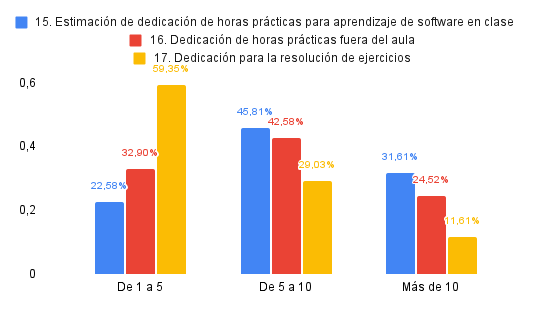
\includegraphics[width=0.8\linewidth]{Fig2.png}
\caption{Valoración del tiempo empleado por parte del alumnado.}
\label{fig2}
\source{Elaboración propia.}
\end{minipage}
\end{figure}

Del mismo modo, en la identificación del tiempo que el alumnado dedica a resolver un ejercicio en el aula, los datos muestran que un 35,4~\% opina que son necesarias dos sesiones, frente a una sesión (16,2~\%), tres sesiones (11~\%) y más de tres (2,7~\%). En conexión con lo anterior, los resultados sugieren que existe una relación significativa entre el tiempo de práctica en el aula en relación con el conocimiento de la interfaz del usuario. En este sentido, aquellos que practican entre 5 y 10 horas lectivas en el aula, tienden a comprender en mayor medida la interfaz del usuario ($\chi^{2}(2,N=154)=6.458$, $p=0.040$). Estos datos se refieren a la relación de tiempo existente entre el planteamiento formativo que está presente en el programa de la asignatura (aportado anteriormente) y que valida el profesor, en oposición con la percepción que tiene el alumnado respecto a sus necesidades formativas. Esta relación es extrapolable a cualquier asignatura con necesidad de formación técnica, ya que no es tanto el hecho concreto sobre un determinado ejercicio sino la comparativa en la percepción del tiempo por parte del profesorado y alumnado.

De igual manera, la forma en la que trabajan en clase (individual o en parejas), está relacionada con el nivel de conocimientos alcanzados. Así, según lo observado, los que trabajan en parejas (52,6~\%), apenas logran un nivel suficiente de conocimiento alcanzado ($\chi^{2}(6,N=154)=15.911$, $p=0.014$). Sin embargo, los datos, reflejados en la \Cref{tab-05}, muestran que el trabajo en parejas es el que prevalece o prefieren, en contraste con el trabajo individual (43~\% vs. 13~\% respectivamente).

%Tabla 5
\begin{table}[htpb]
\centering\small
\begin{threeparttable}
\caption{Relaciones significativas con el trabajo individual o en parejas}
\label{tab-05}
\begin{tabular}{p{5cm}*{4}{l}}
\toprule
Variable &	Opinión & individual & Parejas & Prueba de asociación\\
\midrule
\multirow[t]{3}{=}{Nivel de conocimientos alcanzado con el software enseñado} & Suficiente & 10,3~\% & 52,6~\% & \begin{tabular}[t]{@{}l@{}}$\chi^{2}(6,N=154)=15,911$ \\ $\rho= .014$\end{tabular} \\
  & Bueno & 21,4~\% &	38,1~\% & \\
  & Preferencia & 13,0~\% & 43,0~\% & \\
\bottomrule
\end{tabular}
\source{Elaboración propia.}
\end{threeparttable}
\end{table}

\subsection{Resolución de ejercicios y ayuda complementaria}\label{sec-secoes}
Esta categoría de análisis se centró en la disponibilidad del software visto en la asignatura, así como en el empleo y necesidad de ayuda o tutoriales explicativos. Según se aprecia en la \Cref{fig3}, los resultados muestran un 97,4~\% de opinión positiva en cuanto a la necesidad de disponer fuera del aula de las licencias de los programas vistos en la asignatura. La respuesta mayoritaria hace evidente la importancia para el alumnado de poder disponer de los programas a título individual para completar en forma de autoaprendizaje la formación realizada en el aula.

\begin{figure}[h]
\centering
\begin{minipage}{.8\textwidth}
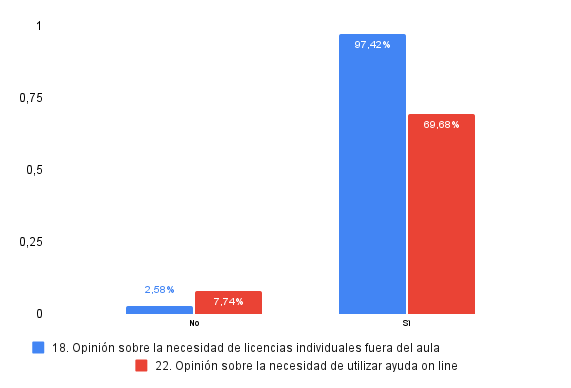
\includegraphics[width=\linewidth]{Fig3.png}
\caption{Valoración de medios de aprendizaje por parte del alumnado.}
\label{fig3}
\source{Elaboración propia.}
\end{minipage}
\end{figure}

De igual forma, respecto al tipo de apoyo que prefiere el alumnado a la hora de resolver un ejercicio práctico planteado en la asignatura, los resultados evidenciaron que en un 45,1~\% prefieren “buscar tutoriales en Internet”. Lo anterior, es seguido por “consultar a un compañero”, con un 26,15~\%, y “preguntar al profesorado”, con un 24,2~\%. Estos resultados ofrecen un indicio claro de la preferencia de los estudiantes consultados a la hora de localizar información de ayuda complementaria, prevaleciendo como se indica, el modelo basado en el autoaprendizaje. 

En coherencia con lo anterior, y referente a los tipos de tutorial explicativo que emplean para completar la explicación de los programas que hace el profesorado en el aula, la evidencia muestra el convencimiento sobre la necesidad de usar tutoriales para el aprendizaje de los programas vistos en la asignatura. Aquí, con un 69,5~\% los datos sugieren que el estudiantado prioriza mayoritariamente el uso de los tutoriales en formato vídeo. Así mismo, los resultados muestran que en su gran mayoría (69,5~\%) consideran necesario disponer de una ayuda \textit{online} para mejorar el aprendizaje de los programas utilizados en la asignatura. 

En esta misma línea de análisis, el hecho de comprender la interfaz de usuario está relacionado significativamente con la conveniencia de tener o buscar ayuda \textit{online} para un mejor aprendizaje del software. En el presente caso, el 62~\% de los estudiantes que entienden bien la interfaz, también consideran conveniente tener ayuda \textit{online} ($\chi^{2}(1,N=154)=5.119$, $p=.024$). Del mismo modo, la mayoría de la muestra que considera conveniente tener ayuda de tutoriales explicativos \textit{online} para su aprendizaje, emplean los formatos que combinan vídeo y audio (49.5~\%). Los datos resultantes muestran que estimar necesario el uso de tutoriales \textit{online}, está significativamente relacionado con un autoaprendizaje mediante formatos en los que prevalecen el vídeo, el audio y el texto ($\chi^{2}(3,N=154)=15.484$, $p=.001$.)

\section{Discusión}\label{sec-format-simple}
La hipótesis que ha sustentado este trabajo plantea como necesaria una evolución hacia las metodologías autoformativas de aprendizaje como estrategia complementaria para la adquisición de conocimiento, desarrollo y perfeccionamiento práctico. A tenor de los resultados obtenidos, se valida la necesidad de profundizar en el desarrollo de tecnologías y metodologías que ahonden en este sentido. Esta evolución en el aprendizaje de herramientas técnicas específicas del entorno audiovisual conlleva un cambio de paradigma en la construcción y articulación de los planes docentes de las diferentes Universidades que imparten el Grado de Comunicación Audiovisual o similares.

Por ello, conforme a los resultados del estudio, el conocimiento solvente de herramientas técnicas junto a la competencia en el manejo de diversos \textit{softwares} de producción audiovisual, resultan esenciales para la muestra seleccionada de cara a la obtención de los objetivos formativos de la asignatura analizada. Sin duda, esta integración de las tecnologías de la información puede enriquecer el proceso de aprendizaje y promover la colaboración, manifestando mejoras notables en términos de participación, motivación y compromiso en sus interacciones con las diversas categorías de \textit{software} empleadas en su trayectoria académica.

Otro aspecto reseñable derivado del estudio es que, dentro de la operativa tecnológica, el alumnado concede un valor especial al tiempo dedicado al pensamiento para la resolución de problemas. En general, la forma en que perciben el tiempo de formación de la tecnología en el aula es baja y creen que el desarrollo de estos conocimientos fortalece tales habilidades). De igual manera, los resultados demuestran que el estudiantado posee habilidades técnicas, de gestión, de información, comunicación, colaboración, creatividad, en el uso del \textit{software} y de las tecnologías digitales, acorde con las llamadas “habilidades digitales del siglo XXI” \cite{van_laar_relation_2017}. De hecho, posiblemente la percepción generalizada de los profesionales en torno a las TIC, es que son vitales en el desarrollo de competencias fundamentales para su ejercicio profesional, fruto de nuevos modelos educativos que combinan el trabajo autónomo a través de plataformas online y las estrategias de trabajo compartido mediados por procesos interactivos que permiten tener acceso a la información y poder transferirla \cite{alcala_del_olmo_fernandez_competencias_2020}.

En este sentido, los hallazgos muestran la necesidad que tendría la Universidad y las Facultades de Comunicación de introducir las tecnologías digitales con el fin de transformar e innovar los procesos educativos \cite{urcid_puga_autoaprendizaje_2022} y estar en conexión con los cambios tecnológicos \cite{falco_reconsiderando_2017}, contemplando también el ofrecimiento de alternativas didácticas al estudiantado para que éstos interactúen y pongan en práctica otras formas de mediación tecnológica \cite{pastor-rodriguez_pildoras_2022}. Lo anterior, también acorde con la obligatoriedad de preparar al alumnado para que, a través del aprendizaje de herramientas tecnologías puedan incorporar interactividad, movilidad, documentación y profundidad, en sus creaciones comunicativas \cite{lopez-garcia_mobile_2019}. A su vez, los resultados acreditan las competencias que puede desarrollar el estudiantado mediante su aprendizaje autónomo, gestionando considerablemente el uso del tiempo, dedicado a planificar, controlar y evaluar sus propios avances sin la necesidad del profesor y con la utilización de tutoriales. Esto coincide con la hipótesis de esta investigación y de otros estudios, sobre la necesidad de estimular la capacidad de competencias en autoaprendizaje como herramienta para la vida profesional y académica. Lo anterior, en línea con la gestión eficaz del tiempo y la proactividad, como variables indispensables en los procesos de autoaprendizaje, soportados también por los recursos tradicionales y las posibilidades que ofrecen las nuevas tecnologías para el aprendizaje \textit{online} \cite{medina-labrador_effects_2023}.

Del mismo modo, para la gran mayoría de la muestra, el autoaprendizaje en esta asignatura está relacionado con la utilización de ayuda \textit{online} a través de tutoriales explicativos vinculados a procedimientos técnicos. Acorde con \textcite{padilla_aprendizaje_2020}, la facilidad para el acceso a tecnologías de la información y a estos tutoriales, conlleva un compromiso mayor para el logro de sus objetivos educativos y la creencia de poder lograr con éxito sus metas académicas. A través de estos, el estudiantado gestiona su propio ritmo de aprendizaje de acuerdo con sus particularidades psicográficas, además de la posibilidad de acceso debido a su gratuidad o bajo coste. Por tanto, es necesario enfatizar la importancia del aprendizaje autónomo como solución a los problemas estructurales existentes en este tipo de asignaturas tecnológicas, y como medio potenciador para la formación, preparación y capacitación profesional del alumnado. En efecto, la autoformación es extrapolable al contexto profesional, productivo y social, obligando a que los individuos tengan la capacidad de adaptarse y adquirir autónomamente nuevas habilidades necesarias para su vida profesional, acordes con la dinámica tecnológica que integra al individuo en grupos sociales, organizaciones, instituciones y empresas. Sin duda, este es uno de los hallazgos más relevantes del estudio, el que demuestra que el estudiantado está adquiriendo, de forma autónoma, competencias en diferentes herramientas tecnológicas que les permitirán la consecución de metas académicas y profesionales. Probablemente, el desarrollo de herramientas como la Inteligencia Artificial, en la que es necesario profundizar y delimitar su utilidad para el aprendizaje autónomo \cite{artiles_rodriguez_agente_2021}, permita al alumnado tener a su disposición nuevas y mejores formas de gestión de su autoaprendizaje conforme a ritmos y tiempos personalizados, complementando y fortaleciendo los métodos, pedagogías y didácticas tradicionales de enseñanza – aprendizaje.

\section{Conclusiones}\label{sec-links}
De acuerdo con los objetivos del estudio, para el alumnado participante resulta esencial el conocimiento y aprendizaje de las distintas tecnologías vinculadas con la producción audiovisual, lo cual está directamente relacionado con factores que intervienen en el nivel de competencias adquiridas, y con el desarrollo de los trabajos académicos realizados. No obstante, el propio diseño curricular se convierte generalmente en una limitación operativa que dificulta los objetivos de enseñanza-aprendizaje. Por ello, las dinámicas propias de este proceso pueden convertirse en retos institucionales al verse limitadas por variables como la temporalidad de la asignatura, la complejidad de los programas, el número de matriculados, los recursos tecnológicos y formación previa del estudiantado. Así mismo, el desarrollo de la tecnología exige constantes procesos de actualización que obligan al alumnado a optar por mecanismos de autogestión, que le permitan aprovechar plenamente las bondades de estas herramientas tecnológicas \cite{granados_maguino_tecnologien_2020}. De hecho, ellos mismos reconocen el valor de las TIC en su educación, especialmente en el desarrollo de habilidades como el aprendizaje autónomo, la comunicación, la investigación y la interacción. Además, consideran que estas tecnologías contribuyen al logro de objetivos profesionales, facilitando el aprendizaje individual e interpersonal, mejorando el trabajo en equipo \cite{espinel_armas_tecnologien_2020}.

Por otro lado, la evolución tecnológica exige al profesorado la utilización de dispositivos que aprovechan la innovación digital, permitiendo una mejor interacción y   seguimiento del proceso de enseñanza-aprendizaje. Por tanto, a pesar de que los cambios curriculares son procesos dispendiosos que pueden demorarse, es relevante que las universidades propongan una adaptación eficaz a la tecnología para integrar curricularmente las demandas del desarrollo profesional \cite{manfredi_sanchez_innovacion_2019}. Evidentemente se observa un distanciamiento entre lo que se enseña en las instituciones educativas y lo que esperan los sectores productivos, que demandan la digitalización como fuente de nuevas oportunidades de empleo \cite{moliner_tecnologiy_2021}, directora de Sostenibilidad de ManpowerGroup, en Avances. Sin embargo, esta implementación tecnológica exige su incorporación efectiva, lo que no siempre está al alcance de las instituciones universitarias. Esto se convierte en un importante punto de investigación para el entorno educativo, toda vez que el simple hecho de adoptar nuevas tecnologías no es adecuado por sí solo. Los modelos educativos actuales necesitan integrar estas tecnologías de manera efectiva, en donde se fomente la innovación a través de estrategias que propendan por el aprendizaje autónomo, acelerado y creativo. Lo anterior, con la responsabilidad del ejercicio docente en cuanto a generar pedagogías y didácticas innovadoras que garanticen la inmersión del estudiantado en las actuales sociedades del conocimiento \cite{falco_reconsiderando_2017}. Evidentemente la utilización de las TIC, son fundamentales porque aseguran la constante adquisición de conocimientos, así como el desarrollo de competencias para la autogestión y el autoaprendizaje del estudiantado. Esto a su vez facilita las dinámicas en la sociedad del conocimiento por el acceso ilimitado e inmediato de información, impulsando así la innovación \cite{urcid_puga_autoaprendizaje_2022}, y que a su vez es inherente a que gran parte de la comunidad universitaria está compuesta por alumnado que se caracteriza por su capacidad para el uso autónomo de dispositivos y nuevas tecnologías digitales, desde temprana edad y desde los primeros años de educación media \cite{mesa_rave_escenarios_2023}, haciéndolas parte de su cotidianidad \cite{granados_maguino_tecnologien_2020}.

Otra conclusión para considerar es la aceptación y valoración positiva por parte de los participantes respecto a la responsabilidad con su propio aprendizaje, asumiendo un mayor índice de implicación, dado que el aprendizaje autónomo requiere más iniciativa proactiva \cite{shao_spatio-temporal_2020}. El estudiante demanda explorar e innovar en los procesos cognitivos de formación relacionados con la interacción tecnológica y el trabajo en equipo. En un primer estadio, es necesario proponer metodologías que permitan emplear el tiempo de clase en actividades que favorezcan el desarrollo de procesos de pensamiento complejos, y de esta manera poder aumentar el trabajo autónomo y la independencia de los estudiantes \cite{suryawan_development_2021}. Esto, simultáneamente con las otras posibilidades didácticas. Por ejemplo, el aprendizaje basado en problemas y la oportunidad de trabajo en equipo, que ayudan a consolidar los conocimientos de manera más amplia, inculcando al alumnado la idea de que son ellos quienes deben responsabilizarse de su propio progreso educativo \cite{pinats_autoaprendizaje:_2023}.

Finalmente, y dadas las limitaciones del presente estudio, es necesario seguir investigando en torno a la relación de las nuevas tecnologías y el desarrollo de competencias para el autoaprendizaje, en jóvenes estudiantes, tanto en el contexto de la educación media como en la universitaria. Es evidente la importancia de analizar y estudiar poblaciones de estudiantado que evidencien diferencias comparativas a nivel de centros educativos y demás aspectos psicográficos, demográficos e interculturales.  

\section{Financiación}
Proyectos Santander-UCM (PR44/21-29919).

\printbibliography\label{sec-bib}
%conceptualization,datacuration,formalanalysis,funding,investigation,methodology,projadm,resources,software,supervision,validation,visualization,writing,review
\begin{contributors}[sec-contributors]
\authorcontribution{Alberto Luis García García}[conceptualization,projadm,funding,supervision,writing]
\authorcontribution{Manuel Sánchez Cid}[conceptualization,investigation,writing,review]
\authorcontribution{Fernando Marroquín-Ciendúa}[conceptualization,formalanalysis,investigation,methodology,writing]
\end{contributors}
\end{document}
